\documentclass[twocolumn]{article}

% Language setting
% Replace `english' with e.g. `spanish' to change the document language
\usepackage[english]{babel}
\usepackage{cite}
\usepackage{physics}
% Set page size and margins
% Replace `letterpaper' with `a4paper' for UK/EU standard size
\usepackage[letterpaper,top=1.75cm,bottom=1.75cm,left=1.75cm,right=1.75cm,marginparwidth=1cm]{geometry}
% Useful packages
\usepackage{amsmath}
\usepackage{graphicx}
\usepackage[usenames,dvipsnames]{xcolor}
\usepackage[colorlinks=true, allcolors=blue]{hyperref}
\usepackage{listings}
\lstset{frame=tb,
  language=Python,
  aboveskip=3mm,
  belowskip=3mm,
  showstringspaces=false,
  columns=flexible,
  basicstyle={\small\ttfamily},
  numbers=none,
  numberstyle=\tiny\color{gray},
  keywordstyle=\color{blue},
  commentstyle=\color{OliveGreen},
  breaklines=true,
  breakatwhitespace=true,
  tabsize=3
}
\usepackage[export]{adjustbox}
\usepackage{booktabs}



\newcommand{\titreproposefr}{Le titre}
\newcommand{\titreproposeen}{The title}
\newcommand{\themefr}{Le thème en une phrase.}
\newcommand{\themeen}{The theme in one sentence.}

\author{Natalie Tsang}
%\newcommand{\coredac}{mon ou ma co-redacteur·rice}

\title{BackPropagation in Neural Networks, a Multilayer Perceptron Implementation}

\begin{document}
\begin{titlepage}
  \centering
  \vskip 60pt
  \LARGE \textbf{BackPropagation in Neural Networks, a Multilayer Perceptron Implementation} \par
  \vskip 6em
  \begin{figure}[h!]
  
\includegraphics[scale=1.25, center]{waterloo_logo.png}  \end{figure}
  \textbf{Department of Mechanical and Mechatronics Engineering}
  \vskip 5em
  \large A Report Prepared For: \par
  \large MTE203
  \vskip 7em
  \large Natalie Tsang \par
  \vskip 1.5em
  \today
\end{titlepage}

\section{Introduction}

\subsection{What are Neural Networks and why use BackPropagation?}
Neural networks are a powerful tool used for machine learning and artificial intelligence. They are created to model the human brain and its biological human neurons. \cite{gursen} Each neuron may have connections to several other neurons in different layers, sending data to nodes in layers above and receiving data from layers beneath. This is loosely modelled on the process where brain neurons receive stimulus, change them using synaptic weights, sum them and produce an output. \cite{gursen} There are different types of artificial neural networks that can be used for machine learning, ranging in complexity and effectiveness. This paper will focus mainly on a multilayer perceptron implementation of a neural network as it is the simplest feed-forward neural network, meaning there are not backwards connections between neurons. To use a neural network for machine learning applications such as image classification, the network must be trained. In brief, the network trains itself by learning the patterns of data samples and which label they belong to. One of the key steps of training is backpropagation which allows the multilayer perceptron to
learn through minimizing measurement costs between predicted outputs and actual outputs. \cite{popescu} Backpropagation algorithms are typically applied after the initial feed forward step, where data is fed into the neural network and a cost function for each node is found. The cost function is found Given the cost functions are all differentiable, costs can be minimized through calculating the gradients of each cost function and updating weights and biases accordingly. Using a backpropagation algorithm during the training of a neural network ensures that the network is attuned to complex features in the data and reduces overall cost. 
\subsection{Introduction to Project and Application}
The multilayer perceptron implementation is one of the more basic neural networks, especially when there are not many layers involved. While other neural networks, such as convolutional neural networks and recurrent neural networks also use backpropagation algorithms to train their networks, multilayer perceptrons are a straightforward neural network for which a backpropagation algorithm can be implemented. The main application focus in this paper will be using a neural network with backpropagation to classify images. Both convolutional neural networks and multilayer perceptrons can be used for problems such as image classification, but  convolutional neural networks take in a 2-dimensional input whereas multilayer perceptrons take in vector inputs. Vector inputs are simpler to work with, and when not working with extremely complex images, can still be effective. In this example of using a multilayer perceptron to classify images, the MNIST dataset \cite{lecun2010mnist} will be used. The MNIST dataset is a collection of handwritten numbers, with corresponding labels to numbers. It is used to identify handwriting, and parse correct numbers from handwriting. This application is useful for scanning documents, turning pictures to text, auto-grading, and many other useful real-world applications.  
\section{Background Information}
\subsection{Neural Networks}
The primary element of a neural network are the artificial nodes, or neurons, that mimic how brain neurons receive stimulus. As opposed to stimulus, artificial neurons receive weighted input signals and produce an output signal.\cite{gursen} These input signals can be mathematically represented by an array of numbers, which are derived from the dataset fed into the network. In the case of an image classification problem, the values might represent pixels of an image. \cite{nielsen1} Neurons are arranged in a network of layers, which can be visualized as rows of nodes. Each single node on a layer is connected to every node on the next layer, but there are no connections between nodes on the same layer. \cite{nielsen1} The first layer of the neural network is the input layer, and contains the input vector. Next, are a number of hidden layers, which can contain any number of neurons. The number of hidden layers in a neural network also varies. The final layer is the output layer, which contains the same number of nodes as there are classes or labels of data. In the case of the MNIST dataset \cite{lecun2010mnist}, the output layer should have 10 nodes, corresponding to the 10 digits. Starting at the input layer, which receives the input vector, an activation function is applied and fed forward to the first hidden layer by applying a weighted connection between the units. This is repeated to the next hidden layers, and after enough iterations, the output layer is achieved.\cite{reid} The net summation of incoming layers, otherwise called the pre activation $z_{i}$ can be described by the following equation: 
\begin{equation}z_{i} = \sum_{i}w_{i}x_{i}+b_{i}
\end{equation}
here $x$ represents the inputs to the function, $w$ represents the weights associated with connections between neurons on one layer to another. \cite{reid}  The $b$ term is the unit's bias value which helps to determine activation of the neuron if there is no input. Next, an activation function will be used to calculate whether or not the neuron should be activated. An activation function that will be used for backpropagation should be differentiable. \cite{tom} There are a few different activation functions that can be used to decide the activation of a neuron, with the most common being non-linear activation functions. A popular non-linear activation function that will be used for testing the neural network in this paper is the sigmoid function, which is used in logistic regression.\cite{reid} The sigmoid function, $\sigma(z)$:
\begin{equation}
\sigma(z) = \frac{1}{1+e^{-z}}
\end{equation} 
will always return a value between 0 and 1. \cite{tom} Applying this activation function to the pre-activation summation, will produce an equation for the unit's activation, $a$ as: 
\begin{equation}a = \sigma(\sum_{i}w_{i}x_{i}+b_{i}).\end{equation}
Applying this function to each layer, will compute the next layer of the network and eventually finish by computing the output vector. Prior to computing the activation of each layer and the output layer, the neural network has a target output that it is trying to match with, as this target represents the correct classes and labels that are associated with each image in the dataset. When split up into units of a neural network, the goal of the network is to map the input vector to output vector accurately so that the computed output vector matches the actual predetermined output vector with as much precision as possible. \cite{reid} To evaluate the accuracy of the network, the difference, $\delta$, between the target output data, $t_{j}$, and computed output data, $a_{j}$, is:
\begin{equation}
    \delta_{j} = t_{j} - a_{j}.
\end{equation}
This equation can be further used to evaluate the cost function, $\varepsilon$, which measures the discrepancy between the target and computed output vector\cite{martens}, and is defined by:
\begin{equation}
    \varepsilon = \frac{1}{2}\sum_{j=1}^{J}\left (\delta_{j}  \right )^{2}=\frac{1}{2}\sum_{j=1}^{J}\left (t_{j} - a_{j} \right )^{2}
\end{equation}
where $j$ represents the total number of units in the output layer, and should be equal to the total number of classes or labels of the dataset. Seeing as the most accurate neural network should have the lowest possible cost, the network can be optimized by determining the minimum of the cost function. This can be found by computing the gradient of the cost function to find direction of descent. \cite{jorge}
\subsection{Backpropagation Algorithm}
This leads to the backpropagation algorithm, which is used to update the connections' weights and biases which are important to the activation function. These weights are often initialized randomly to non-zero values, and through the process of backpropagation are tuned based on the differing output and target data to increase accuracy. Using backpropagation is a straightforward and effective method for propagating information regarding the computed output to the inputs, so that they can adjust accordingly and produce a more accurate output in subsequent updates. \cite{lisbon} As it was mentioned above, recalculating weights of the network are related to determining the direction of the steepest descent. The function for the next weight, $w(t+1)$, can be found using this relationship between the previous weight $w(t)$ and the weight step, $\Delta w(t)$:
\begin{equation}
    w(t+1) = w(t) + \Delta w(t).
\end{equation}
Determining the weight step typically requires computation of the cost gradient, which is the partial derivative of the cost function with respect to weight. \cite{reid} There are two specific cases that must be addressed when implementing a backpropagation algorithm, the first being when computing the partial derivative for an output layer unit and the second for when computing the partial derivatives for the hidden layer units. Generally, the chain rule can be used when computing the partial derivative, $\frac{\partial \varepsilon  }{\partial w}$. Above in (4), difference ($\delta$) is a function of $t$ and $a$, and in (3), activation ($a$) is a function of $w$, $x$ and $b$. The chain rule for partial derivatives can be used to define:
\begin{equation}
    \frac{\partial \varepsilon  }{\partial w} =  \frac{\partial \varepsilon  }{\partial a} \cdot  \frac{\partial a  }{\partial w}
\end{equation}
which can be used through repeated application to compute the gradient for each weight in the network. \cite{reid} When computing the partial derivative, $\frac{\partial \varepsilon }{\partial w}$, for a neuron in the output layer, the equation is simpler and can be solved as:
\begin{equation}
        \frac{\partial \varepsilon }{\partial a} =  \frac{1}{2}\frac{\partial (t-a)^{2}  }{\partial a} = -(t-a)
\end{equation}
which gives the negative value of the computed output data subtracted from the target output data. Alternatively, if the unit is not in the output layer, and it is instead in one of the hidden layers, computing the partial derivative of $\frac{\partial \varepsilon }{\partial w}$ involves a summation of all the units, $k$ that the current unit is connected to by a non-zero weighted connection. This is because the cost function, $\varepsilon$, is dependent on the activation, $a$, for all $k$ units that the current unit, $j$, is connected to. Then:
\begin{equation}
        \frac{\partial \varepsilon }{\partial a_{j}} = \sum_{k=1}^{K} \frac{\partial \varepsilon}{\partial a_{k}}\frac{\partial a_{k}  }{\partial a_{j}} 
\end{equation}
where separating the term $\frac{\partial a_{k}  }{\partial a_{j}} $ can be solved as
\begin{equation}
        \frac{\partial a_{k} }{\partial a_{j}} = w_{kj}\sigma'(z_{j})
\end{equation}
which gives 
\begin{equation}
    \frac{\partial \varepsilon }{\partial a_{j}} = \sum_{k=1}^{K} \frac{\partial \varepsilon}{\partial a_{k}} w_{kj}\sigma'(z_{j}).
\end{equation}
The term $\frac{\partial \varepsilon}{\partial a_{k}}$ can be computed prior to the backwards propagation of cost information, and assumes that computation begins at the output layer and then moves on to the hidden layers. \cite{reid} Returning to (8), the term $\frac{\partial a}{\partial w}$ can be solved for, 
\begin{equation}
    \frac{\partial a}{\partial w} = \frac{\partial a}{\partial z} \frac{\partial z}{\partial w} = \sigma'(z)a
\end{equation}
thus finishing the computation of the gradient, $\grad \varepsilon = \frac{\partial \varepsilon}{\partial w}$. \cite{reid} Once  the derivatives for all the nodes in the network have been computed, each weight can be updated. This involves using the rule that was looked at in (6), which is a function for determining the next weight. This technique, called gradient descent, calculates a weight step in the direction opposite to the gradient of cost and scaled by the constant learning rate value. A learning rate value must be pre-determined prior to making any backpropagation calculations, and is consistent across the whole network, and the layers. Further solving (6), using the gradient descent technique gives
\begin{equation}
    \Delta w(t) = - \eta \grad \varepsilon(w) = - \eta \frac{\partial \varepsilon}{\partial w}
\end{equation}
and when solving for the next weight, $w(t+1)$ produces
\begin{equation}
    w(t+1) = w(t) - \eta \frac{\partial \varepsilon}{\partial w}
\end{equation}
where $\eta$ is the learning rate, and $\grad \varepsilon(w)$ is the gradient of the cost function with respect to weights. \cite{reid} Determining an adaptive equation for biases, which are all initially set to 0, takes a similar form to the update equation for weights. Updating biases in addition to updating weights are important, as it can increase the model's ability to adapt during the training stage. Similar to updating the weights, the cost function, $\varepsilon$, can be used to compute the partial derivative with respect to the bias $b$.\cite{zhang} The bias adaptation function also involves gradient descent, 
\begin{equation}
    b(t+1) = b(t) + \Delta b(t) = b(t) - \eta \frac{\partial \varepsilon}{\partial b}
\end{equation}
and similar to the equation for updating the weights, involves minimizing the previous bias value by subtracting the partial derivative of cost with respect to bias multiplied by the learning rate, $\eta$.\cite{zhang} The partial derivative of the cost function in terms of bias is defined as 
\begin{equation}
    \frac{\partial \varepsilon}{\partial b} = \frac{\partial \varepsilon}{\partial z} \frac{\partial z}{\partial b} = \frac{\partial \varepsilon}{\partial z} \frac{\partial}{\partial b} [\sum_{i} w_{i}x_{i}+b_{i}]
\end{equation}
where $\frac{\partial}{\partial b}[\sum_{i}w_{i}x_{i}+b_{i}]$ can be reduced to 1, due to the bias term having a linear relationship with the function Z. \cite{zhang} This simplifies the equation for $\frac{\partial \varepsilon}{\partial b}$ to 
\begin{equation}
    \frac{\partial \varepsilon}{\partial b} = \frac{\partial \varepsilon}{\partial z} = -\delta = a - t
\end{equation} 
where the final computation is equal to computed output data subtracted from the target output data.\cite{zhang} Thus, the final equation for updating biases is 
\begin{equation}
    b(t+1) = b(t) - \eta \sum_{n=1}^{N}(a - t)
\end{equation}
where $n$, where n represents the number of layers. \cite{zhang}With this equation, the biases can now be updated, thus completing the backpropagation algorithm with adaptive weights and biases. 
\section{Approach}
The purpose of this project is to reflect on the importance and effectiveness for using the backpropagation algorithm when training neural networks. More specifically, this application of the multilayer perceptron is to produce correct classifications of handwritten digits. The ability of the multilayer perceptron to classify digits can be quantified as an accuracy percentage that is calculated based on how many images it can correctly predict from the train and test datasets. The multilayer perceptron in this project will be reflective of the equations discussed in the background section, as these equations provide the basis for the code functions for the feed-forward and backward propagation step. The three main functions that will be written for the multilayer perceptron are the \texttt{initialize\_parameters}, \texttt{forward}, \texttt{backward} functions. 
\begin{enumerate}
    \item \texttt{initialize\_parameters} function will be used to set up the neural network using the given layer sizes, random connection weights and biases set to zero.
    \item \texttt{forward} function will be used to calculate the preactivation, $z$, discussed in Equation 1, and using this with the sigmoid function, Equation 2, compute the unit's activation to determine whether or not it should be activated. 
    \item \texttt{backward} function is used during training to calculate how much to update weights and biases based on a gradient descent technique described in section 2.2. 
\end{enumerate}
Seeing as the goal of backpropagation is to fine tune weights and biases through minimizing the cost function, there should be progressively fewer differences between the computed output layer and the actual target output layer when training a network. \cite{nielsen1}  To evaluate whether or not the multilayer perceptron implemented in this project works as expected when using a backpropagation algorithm, the accuracy per training step, and final accuracy with the test dataset will be indicative of the network's precision. Determining how "good" a training or final accuracy can be subjective, as this can change based on the size of the dataset, functions used for the neural network, type of dataset, number of layers used and much more. In general, above an 85\% accuracy is good when training a neural network on the MNIST dataset \cite{lecun2010mnist}, as this is a relatively simple dataset but is being implemented from scratch using Python \cite{5python} with the Numpy \cite{harris2020array} package. The Tensorflow package \cite{tensorflow2015-whitepaper} is used only to load the MNIST dataset, while Matplotlib \cite{Hunter:2007} is used to plot the sample images. Some experiments will be conducted to obtain as high an accuracy as possible; including varying learning rate and number of epochs.
\section{Implementation}
To implement a mulitlayer perceptron using backpropagation in Python \cite{5python} the Numpy \cite{harris2020array} package and Tensorflow \cite{tensorflow2015-whitepaper} package was used. Chat-GPT was also used to generate code \cite{openai_gpt3}, some of which was subsequently edited.
\\\newline
When training a neural network for image classification, a training data set is needed, which contains a separate set of images as the test data set. The main difference between the two data sets is that the training set is typically substantially larger and is a set of training examples used to teach the neural network how to classify images with accuracy. \cite{grosse2} In comparison the test dataset is smaller and is used to verify the accuracy and performance of the neural network. When loading the MNIST dataset, as seen below in Listing 1, the test and train images and labels have already been separated and can be loaded as different objects. The MNIST dataset loaded from Tensorflow \cite{tensorflow2015-whitepaper} contains 60 000 training images and 10 000 test images. The images must be normalized as it helps the training process reach better convergence, as all input data has a similar scale. The specific function \texttt{astype('float32')} ensures that all the input pixels are normalized to the same data type.
\begin{lstlisting}[caption={Importing the MNIST dataset, and parsing the test and training images},captionpos=b]
(train_images, train_labels), (test_images, test_labels) = mnist.load_data()
train_images = train_images.reshape((60000, 28 * 28)).astype('float32') / 255
test_images = test_images.reshape((10000, 28 * 28)).astype('float32') / 255
\end{lstlisting}
An example of the handwritten digits that will be used as input images for the neural network is shown below in Figure 1. These are displayed prior to reshaping or data type normalization.
\\
\begin{figure}[h!]
    \centering
    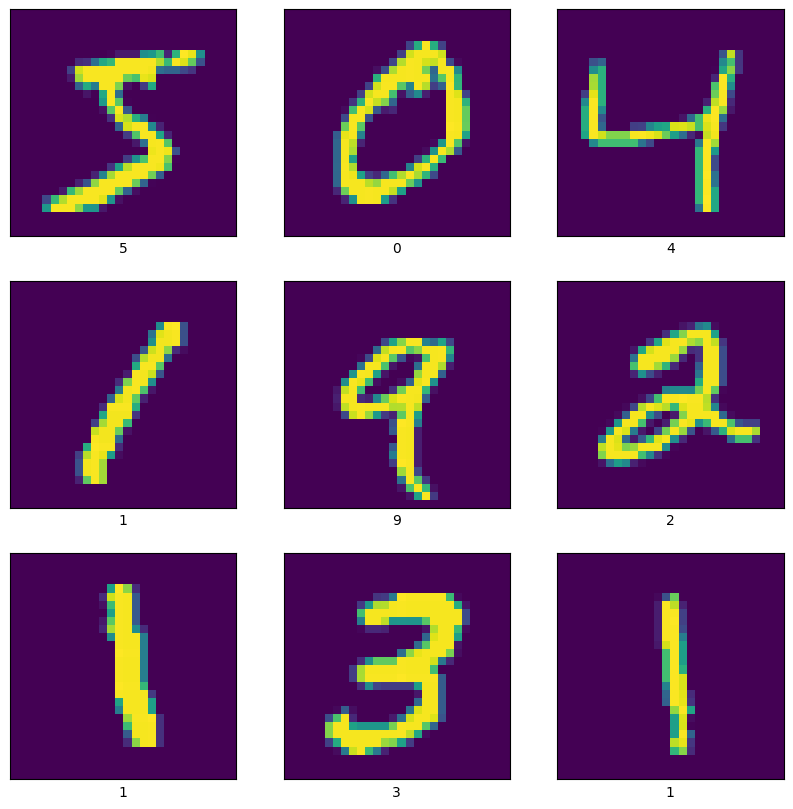
\includegraphics[scale=0.2]{MNIST_sampleset.png}
    \caption{A sampling of the MNIST dataset input images}
    \label{fig:enter-label}
\end{figure}
\\
The next step in the code is to initialize some global variables for the model to use. These include the sizes of the input, hidden and output layers, the learning rate and the number of epochs. In this implementation, the standard image size is 28x28, so the input layer has 784 units (image size flattened) \cite{nielsen1}, the hidden layer is sized down to 128 units, and the output layer has 10 units, corresponding to 10 classes. If more hidden layers are added, the sizes of the new layers would be appended to the array \texttt{hidden\_sizes} in Listing 2. The learning rate, which will be used in the backpropagation algorithm, is used to control convergence \cite{martens} and typically ranges between 0 and 1. After trying learning rates at different increments between 0.01 and 1, it was decided that the learning rate with fastest convergence and minimal noise is 1. The number of epochs in the dataset also contribute to rate of convergence and level of accuracy. Using too many epochs can lead to over-training, and large fluctuation of accuracy, while using fewer epochs can lead to the data being under-trained. For this application, the sizes of 50 - 200 epochs were trialled, and 150 epochs were decided on as it consistently produced the highest accuracy. 
\begin{lstlisting}[caption={Global variable initialization when using the sigmoid activation function},captionpos=b]
input_size = 784  # 28x28 images flattened
hidden_sizes = [128]
output_size = 10  # 10 classes (digits 0-9)
learning_rate = 1
num_epochs = 150
\end{lstlisting}
The next step is to define all of the functions that will be used for the training and testing of the multilayer perceptron. The first function, \texttt{initialize\_parameters} is used to set up the parameters of the neural network and initialize the weights and biases of the network. This function, shown in Listing 3, assigns the weights for each unit per layer to a random variable while assigning the biases to zeros.
\begin{lstlisting}[caption={Determining the initial values of all weights and biases in the neural network},captionpos=b]
def initialize_parameters(input_size, hidden_sizes, output_size):
parameters = {}
layer_sizes = [input_size] + hidden_sizes + [output_size]

for i in range(1, len(layer_sizes)):
    parameters[f'W{i}'] = np.random.randn(layer_sizes[i - 1], layer_sizes[i]) * 0.01
    parameters[f'b{i}'] = np.zeros((1, layer_sizes[i]))

return parameters
\end{lstlisting}
The next function is the sigmoid function that will be later called in the forward function, as this activation function is used to determine the activation of a neuron.
\begin{lstlisting}[caption={The sigmoid function.},captionpos=b]
    def sigmoid(x):
      return 1/(1 + np.exp(-x))
\end{lstlisting}
The \texttt{forward} function represents the feed forward step in multilayer perceptrons. In this step, the pre-activation, $z$, and the activation, $a$, are calculated for every unit in the network at each layer. The pre-activation is a sum of inputs, which requires taking the dot product of the previous layer's activation and the matrix of weights, then adding the bias vector. The weights are represented as a matrix where each row corresponds to the weights of a specific neuron on one layer, and the columns correspond to the weights of a specific neuron on the previous layer, so the intersections represent which neurons are connected and by what weight value. Having computed the value of the pre-activation, the sigmoid function can be applied to determine the activation of the current layer. In code, the feed forward step of the multilayer perceptron can be summarized in Listing 5. 
\begin{lstlisting}[caption={The Feed-Forward function, calculating pre-activation, Z, and activation, A.},captionpos=b]
    def forward(X, parameters):
    cache = {'A0': X}

    for i in range(1, len(parameters) // 2 + 1):
        Z = np.dot(cache[f'A{i-1}'], parameters[f'W{i}']) + parameters[f'b{i}']
        A = sigmoid(Z)
        
        cache[f'Z{i}'] = Z
        cache[f'A{i}'] = A

    return cache
\end{lstlisting}
After the forward step, the backward step must be implemented. This step uses the backpropagation algorithm to compute the gradient of the cost function through the two methods discussed in (8) and (9). The first equation is used to compute the gradient for the output layer, while the latter is used to compute the gradient for the hidden layers. After determining the gradients for cost with respect to weight and biases, the current weights and biases can be minimized and updated. This process is shown below in Listing 6. 
\begin{lstlisting}[caption={Computing the updated weights and biases using the Backpropagation function. Note some non-essential code has been removed but this should not hinder understanding.},captionpos=b]
    def backward(X, Y, cache, parameters, learning_rate):
    # Compute the gradient of the output layer
    dZ = A_output - Y
    dW = np.dot(cache['A' + str(len(parameters) // 2 - 1)].T, dZ) / m
    db = np.sum(dZ, axis=0, keepdims=True) / m
    gradients['dZ' + str(len(parameters) // 2)] = dZ
    gradients['dW' + str(len(parameters) // 2)] = dW
    gradients['db' + str(len(parameters) // 2)] = db

    # Compute the gradient for hidden layers
    for l in range(len(parameters) // 2 - 1, 0, -1):
        dZ = np.dot(gradients['dZ' + str(l + 1)], parameters['W' + str(l + 1)].T) * cache['A' + str(l)] * (1 - cache['A' + str(l)])
        dW = np.dot(cache['A' + str(l - 1)].T, dZ) / m
        db = np.sum(dZ, axis=0, keepdims=True) / m
        gradients['dZ' + str(l)] = dZ
        gradients['dW' + str(l)] = dW
        gradients['db' + str(l)] = db

    # Update weights(parameters) using the gradients
    for l in range(1, len(parameters) // 2 + 1):
        parameters['W' + str(l)] -= learning_rate * gradients['dW' + str(l)]
        parameters['b' + str(l)] -= learning_rate * gradients['db' + str(l)]
    return parameters
\end{lstlisting}
The final \texttt{train} function helps to summarize how \texttt{initialize\_parameters}, \texttt{forward} and \texttt{backward} are used together to train the neural network. In brief, the neural network is initialized, then at each epoch, the forward function step is applied, followed by the backward step. Given the number of epochs, the accuracy was not printed at each increment, but instead at steps of 10.
\begin{lstlisting}[caption={Combininig all of the functions for the Multilayer Perceptron with Backpropagation. Note some non-essential code has been removed but this should not hinder understanding.},captionpos=b]
    def train(X, Y, input_size, hidden_size, output_size, learning_rate, num_epochs):
    parameters = initialize_parameters(input_size, hidden_size, output_size)
    for epoch in range(num_epochs):
        cache = forward(X, parameters)
        parameters = backward(X, Y, cache, parameters, learning_rate)
        if (epoch + 1) % 10 == 0:
            accuracy = np.mean(predicted_labels == np.argmax(Y, axis=1)) * 100
            print(f'Epoch [{epoch + 1}/{num_epochs}], Accuracy: {accuracy:.2f}%, Loss: {loss:.4f}%')
    return parameters

    trained_parameters = train(train_images, train_labels, input_size, hidden_sizes, output_size, learning_rate, num_epochs)
\end{lstlisting}
Finally to ensure accuracy with the test dataset, the \texttt{predict} function, in Listing 7, was written to apply the forward function on an input dataset, thus giving the neural network a dataset that it has not seen before to predict the actual accuracy of the network. Without testing on a separate test dataset, the problem of over-fitting can occur, and the accuracy might be falsely assumed to be much higher than it actually is since the model was only trained on a dataset that it has become familiar with. A very high training accuracy indicates that a network can correctly classify its training images, but when the test accuracy is much lower, is an indication that the network has become effective at memorizing the training set's classifications and is not good at actually classifying all digits. \cite{nielsen2} To avoid this, it is best to train then test on two separate data sets, then compare the two accuracies to make sure that over-fitting of data is not occurring. 
\begin{lstlisting}[caption={The prediction function and its application of the test dataset with the neural network},captionpos=b]
    def predict(X, parameters):
    cache = forward(X, parameters)
    return np.argmax(cache['A2'], axis=1)

    test_predictions = predict(test_images, trained_parameters)
    true_labels = np.argmax(test_labels, axis=1)
    accuracy = np.mean(test_predictions == true_labels) * 100
    print(f'Test Accuracy: {accuracy:.2f}%')
\end{lstlisting}
\section{Results}
\subsection{Train and Test Results}
The training results are the output of the \texttt{train} function when given the input training dataset, using the initial parameters that produced the most optimal results. These initial parameters were a learning rate of 1 and 200 epochs. Looking at the results from the training function, it is evident that with more training the neural network's accuracy increases. The increasing accuracy corresponding to iterations of epochs shows that the backpropagation algorithm works, and that through adapting weights and biases based on the gradient of the cost function the network is able to improve its predictions. To ensure that over fitting of data is not occurring, and that the network can make accurate predictions for any given digits, instead of memorizing quirks of the training data, the test accuracy must be computed. Using the same neural network that produced the training accuracy results in Table 1, the test accuracy was calculated to be \textbf{90.08\%}. Based on how close the values for maximum training accuracy and test accuracy are, the neural network does not show signs of over-fitting and proves to be quite precise when given new data. 
\begin{table}[ht]
\caption{Accuracy results from Training Function}
\label{ta:territory-tabular-both}
\centering
\begin{tabular}[t]{cc} 
\toprule
 \textbf{Epochs} & \textbf{Accuracy (\%)} \\ 
\midrule
    10  &  11.31  \\
    20 & 15.17\\
    30 & 21.72\\
    40 & 33.19 \\
    50 & 47.74\\
    60 & 60.82\\
    70 & 68.93\\
    80 & 73.89\\
    90 & 77.70\\
    100 & 80.95\\
    110 & 83.36\\
    120 & 85.10\\
    130 & 86.33\\
    140 & 87.26\\
    150 & 87.90\\
    160 & 88.44\\
    170 & 88.88\\
    180 & 89.27\\
    190 & 89.52\\
    200 & 89.74\\                               
\bottomrule
\end{tabular}
\end{table}
\subsection{Deciding on Initial Parameters: Learning Rate and Epochs}
Before settling on the previous conclusions for test and train accuracy documented in Table 1 and section 5.1, varying learning rates and epochs were tested. A learning rate of 1 was chosen, as based on Table 1, too small of a learning rate, 0.1, will require many epochs before convergence. Despite general recommendations for learning rates being between 0 and 1, some sources \cite{nielsen2} provided examples of learning rates greater than 1, thus leading to testing a learning rate of 2 as well. Similar to the low learning rate, using a high learning rate also proved to have slow convergence, as in Table 2, the maximum accuracy at this learning rate is 31.91\%. Changing the number of epochs did not have as large of an effect on the test and train accuracy, but the decision to use 200 epochs was chosen as it can achieve an accuracy of over 90\% while not taking too much time, eg. >5minutes. Given that the test accuracy for 250 epochs is slightly higher than the train accuracy, it suggests that the network could be trained using more epochs without over fitting data. This would only incur marginal accuracy increases for significant increases in run-time, which may not be worth it depending on hardware specifications, time restrictions, use cases and the scope of the problem. 
\begin{table}[h!]
\caption{Test and Train accuracy when learning rate and number of epochs are changed. }
\centering
\begin{adjustbox}{width=\columnwidth,center}
\begin{tabular}[t]{ ccccc}
\toprule
 \textbf{\# of Epochs}&\textbf{Learning Rate}&\textbf{Train Accuracy(\%)}&\textbf{Test Accuracy (\%)}&\textbf{Run-time (min)}\\[0.5ex]
 \midrule
150&1&88.07&88.85&3\\[0.5ex]
250&1&90.28&90.92&6\\[0.5ex]
200&0.1&47.08&46.91&5\\[0.5ex]
200&2&39.91&31.92&5\\[0.5ex]
 \midrule
 200&1&49.54&58.80&5\\[0.5ex]
 \bottomrule
\end{tabular}
\end{adjustbox}
\end{table}
\section{Discussion}
When analyzing at the plotted results for the training of the Multilayer perceptron, it is clear that with more iterations, the predictions that the neural network is making are becoming more accurate. This is indicative that the \texttt{backward} function is properly minimizing costs and updating weights and biases. The steepest change in accuracy happens between 20-80 epochs, and this is likely where the weights and biases are updating most drastically. In comparison, between 100-150 epochs, the neural network is still improving its accuracy but at a slower rate. From 150-200 epochs, the weight and bias update, and subsequent increase in accuracy, becomes very minimal but is still increasing. From the results in Table 2, if there were more epochs in the training cycle, it is likely that the accuracy would continue to increase at an even slower rate than the last portion of the graph, representing how the graph would flatten out over time. In Figure 2, it is also clear that there is no noise at the high accuracy, which can be common for some neural networks and may also be a sign of over-fitting. Some future tests that could help determine at which point the model has become over-fitted would be to continue adding more epochs until the graph shows sign of noise at high accuracy or the computed test-accuracy is much lower. Overall, achieving over a 90\% accuracy for recognizing handwritten digits is good, but whether or not this multilayer perceptron could be used in real-world applications depends significantly on the use case. If it were used for automated marking on exams, this would not be precise enough, as 9 in 10 digits might be scanned in wrong, which could lead to a lot of re-marking. On the other hand, if this were used as part of a note-taking app that processes handwriting to text digits, making a few mistakes would be passable as the user would be able to fix these mistakes as they write. 
\begin{figure}[h!]
    \centering
    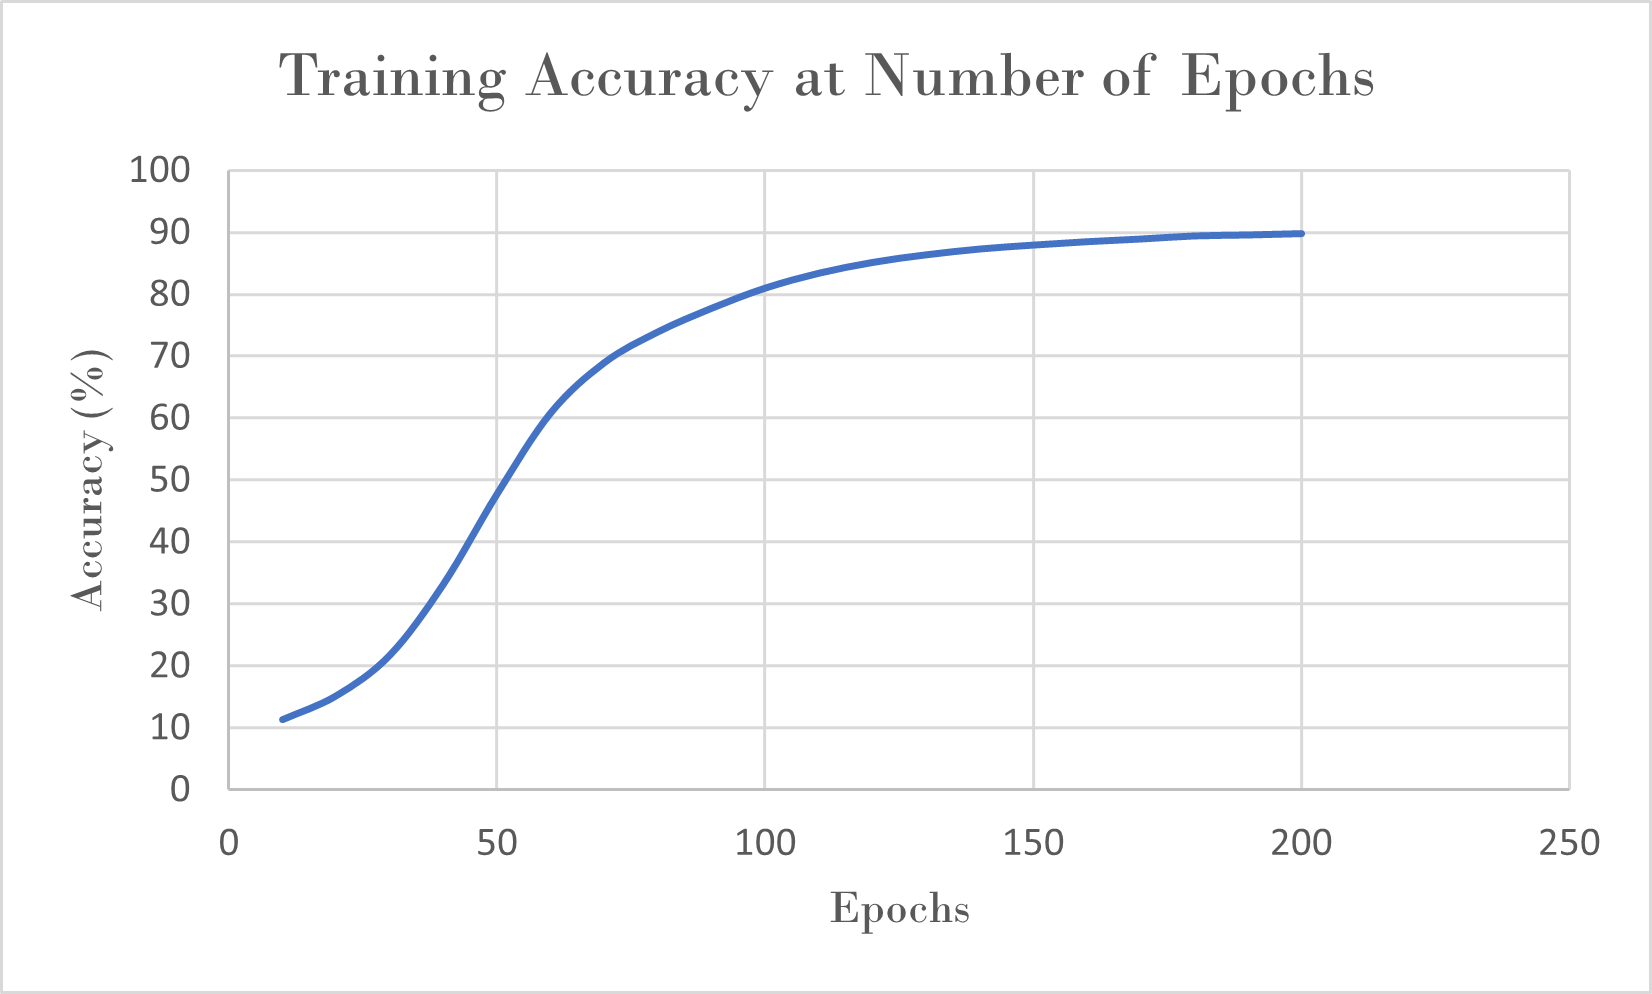
\includegraphics[width=0.95\linewidth]{accuracyvsepoch.png}
    \caption{Plot of Training Accuracy at different Epochs}
    \label{Plot of Training Accuracy at different Epochs}
\end{figure}
\section{Conclusion}
In summary, the multilayer perceptron is an effective neural network to use when classifying simple images. Seeing as the multilayer perceptron is able to achieve over a 90\% accuracy against the both the test and the train dataset, the backpropagation algorithm is demonstrated to be effective at training a neural network and improving accuracy. When compared to the human brain, it is clear that only classifying 9 in 10 numbers correctly is quite low, but for a simple artificial neural network, scoring above an 85\% accuracy indicates a well-trained network. Based on the results in this network, using the sigmoid function as an activation function, updating both weights and biases, and the chosen cost function worked well, but in future research it would be interesting to see if changing the activation function or using a different cost function would affect accuracy. As previously mentioned in the discussion section, a good next step if given more time or fasting computing power would be to add more epochs to see at what point the multilayer perceptron becomes over-fitted. 
\clearpage
\bibliographystyle{IEEEtraN}
\bibliography{ref}

\end{document}
